\documentclass[10pt]{beamer}
\usepackage{subfigure}
\usepackage{amssymb, amsmath, amsfonts,verbatim}
\usepackage{tikz, booktabs}
\usepackage{media9}
\graphicspath{ {./} }
\usetikzlibrary{matrix,arrows,fit,backgrounds,mindmap,plotmarks,decorations.pathreplacing}

\usepackage{pgfplots}
\pgfplotsset{compat=1.12}
\pgfdeclarelayer{background}
\pgfsetlayers{background,main}

\tikzset{decoration={name=none},}

\newlength\figureheight
\newlength\figurewidth

\newcommand{\tikzdir}[1]{#1.tikz}
\newcommand{\inputtikz}[1]{\input{\tikzdir{#1}}}

\newcommand{\tI}{\tilde {\mathcal I}}
\newcommand{\tA}{\tilde A}
\newcommand{\ty}{\tilde y}
\newcommand{\tx}{\tilde x}
\newcommand{\tw}{\tilde w}
\newcommand{\tv}{\tilde v}
\newcommand{\tC}{\tilde C}
\newcommand{\tP}{\tilde P}
\newcommand{\Ic}{{\mathcal I^c}}
\newcommand{\J}{{\mathcal J}}
\newcommand{\K}{{\mathcal K}}

\DeclareMathOperator{\pr}{Pr}
\DeclareMathOperator{\Smin}{Smin}
\DeclareMathOperator{\Smid}{Smid}
\DeclareMathOperator{\Smax}{Smax}
\DeclareMathOperator{\MSE}{MSE}
\DeclareMathOperator{\rank}{rank}
\DeclareMathOperator{\Med}{Med}
\DeclareMathOperator{\Max}{Max}
\DeclareMathOperator{\Min}{Min}
\DeclareMathOperator{\tr}{tr}
\DeclareMathOperator{\Cov}{Cov}
\DeclareMathOperator{\logdet}{log\;det}
\DeclareMathOperator{\argmin}{arg\;min}
\DeclareMathOperator{\argmax}{arg\;max}
\let\Tiny\tiny

\title[Secure Info Fusion]{Secure Information Fusion in Cyber-Physical Systems}
\author[Yilin Mo]{Yilin Mo}
\institute[Tsinghua]{
  Department of Automation\\ Tsinghua University\\
}
\date[Dec 13, 2018]{Dec 13th, 2018 \\ 
  \small Joint Work with Xiaoqiang Ren, Duo Han, Xinghua Liu, Jiaqi Yan,\\
  Prof. Lihua Xie and Prof. Emanuele Garone}

\usetheme[subsectionpage=none,block=fill]{metropolis}
\definecolor{thupurple}{RGB}{102,8,116}
\setbeamercolor{title separator}{fg=black!50}
\setbeamercolor{frametitle}{bg=thupurple!70!black}

\begin{document}

\maketitle 

\section{Introduction}

\begin{frame}{Cyber-Physical System}
  \begin{itemize}
  \item Cyber-Physical Systems (CPSs) refer to the embedding of computation, communication and control into physical spaces.
    \begin{center}
      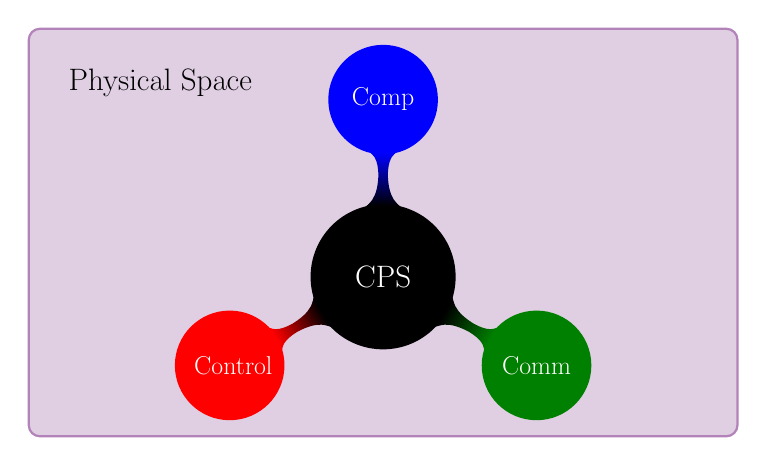
\begin{tikzpicture}[scale=0.45,transform shape,level distance=0cm,
        level 1 concept/.append style={sibling angle=120,minimum size = 3cm},
        ]
        \path [draw=thupurple!50,fill=thupurple!20,thick,rounded corners] (-10,-4.5) rectangle (10,7);
        \node at (-9,6) [anchor=north west] {\Huge Physical Space};
        \path[mindmap,concept color=black,text=white]
        node[concept] {\Huge CPS}
        [clockwise from=330]
        child[concept color=green!50!black] { node[concept](communication) {\huge Comm} }
        child[concept color=red] { node[concept](control) {\huge Control} }
        child[concept color=blue] { node[concept](computation) {\huge Comp} };
      \end{tikzpicture}
    \end{center}
  \item Applications: aerospace, chemical processes, civil infrastructure, energy, manufacturing and transportation. 
  \end{itemize}
\end{frame}

\begin{frame}{Security Threats for the CPS}
  \begin{itemize}
  \item The next generation CPS: Smart Grids, Smart Buildings, Smart Home, Internet of Things, will make extensive use of widespread sensing and networking.
  \item As the CPSs become ``smarter'', they are also more vulnerable to malicious attacks.
  \end{itemize}
  \begin{figure}[ht]
    \centering
    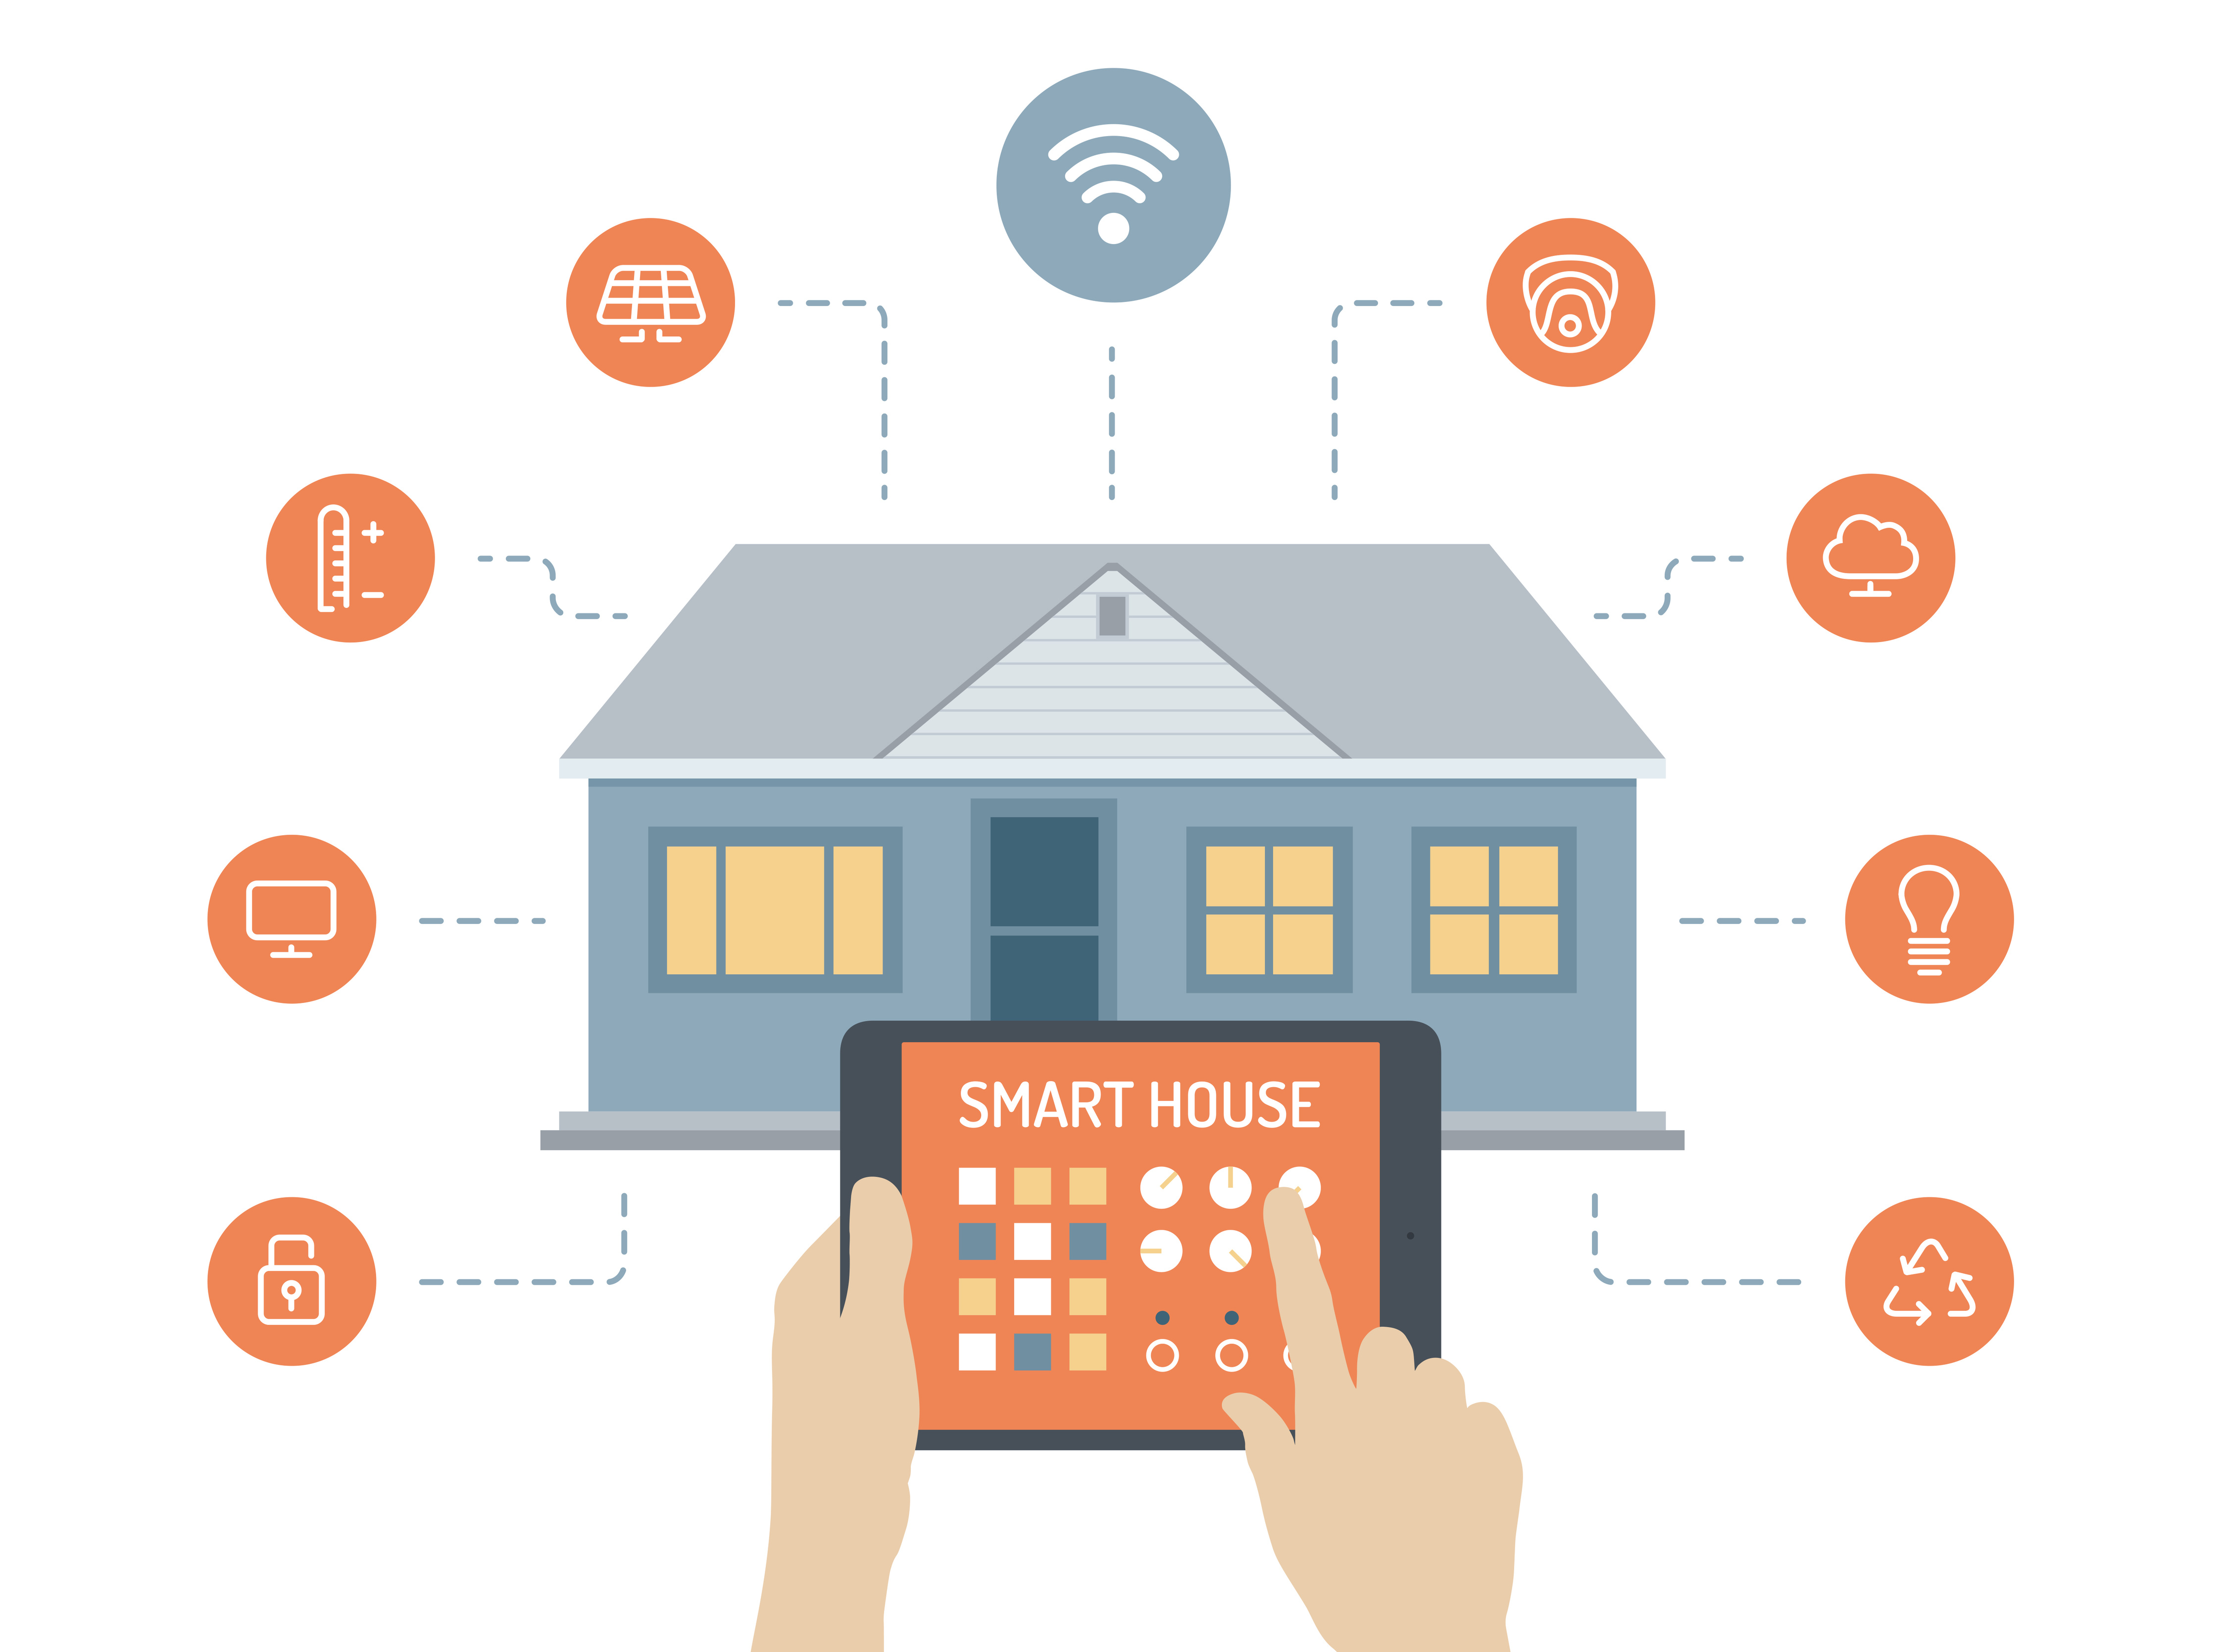
\includegraphics[width=0.6\textwidth]{SmartHome.jpg}
  \end{figure}
\end{frame}

\begin{frame}{Stuxnet}
  \begin{figure}[ht]
    \centering
    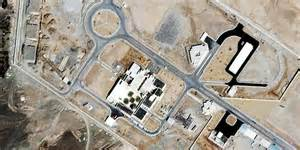
\includegraphics[width=0.8\textwidth]{stuxnet.jpg}
  \end{figure}
  Stuxnet is the first discovered malware that spies on and subverts industrial control systems. It was discovered in June 2010. 
\end{frame}

\begin{frame}{Industrial Control Systems}
  \begin{figure}[ht]
    \centering
    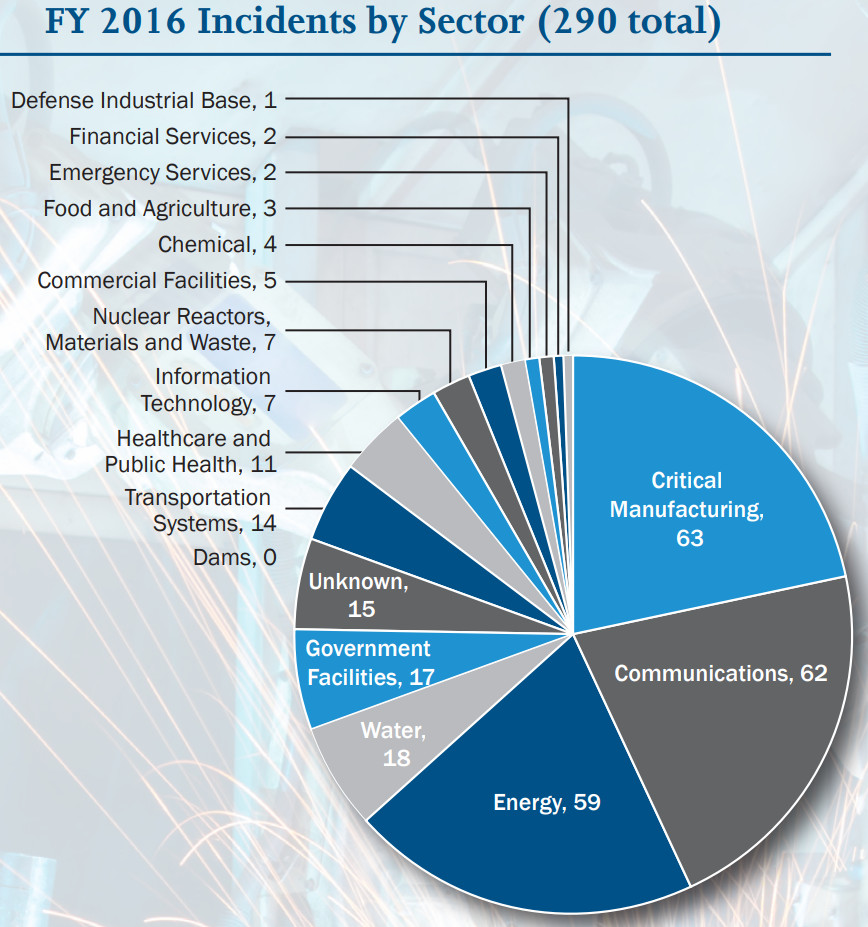
\includegraphics[width=0.6\textwidth]{cert.jpg}
  \end{figure}
  In FY 2016, ICS-CERT (Industrial Control Systems Cyber Emergency Response Team) received and responded to 290 incidents as reported by asset owners and industry partners.
\end{frame}


\begin{frame}{Industrial Control Systems}
  The scope of incidents encompassed a vast range of threats and observed methods for attempting to gain access to both business and control systems infrastructure, including but not limited to the following:
  \begin{enumerate}
  \item  Unauthorized access and exploitation of Internet facing ICS/Supervisory Control and Data Acquisition (SCADA) devices,
  \item  Exploitation of zero-day vulnerabilities in control system devices and software, 
  \item  Malware infections within air-gapped control system networks,
  \item \dots
  \end{enumerate}

\end{frame}

\begin{frame}{Attack Through Compromised Supply Chain}
  \begin{figure}[ht]
    \centering
    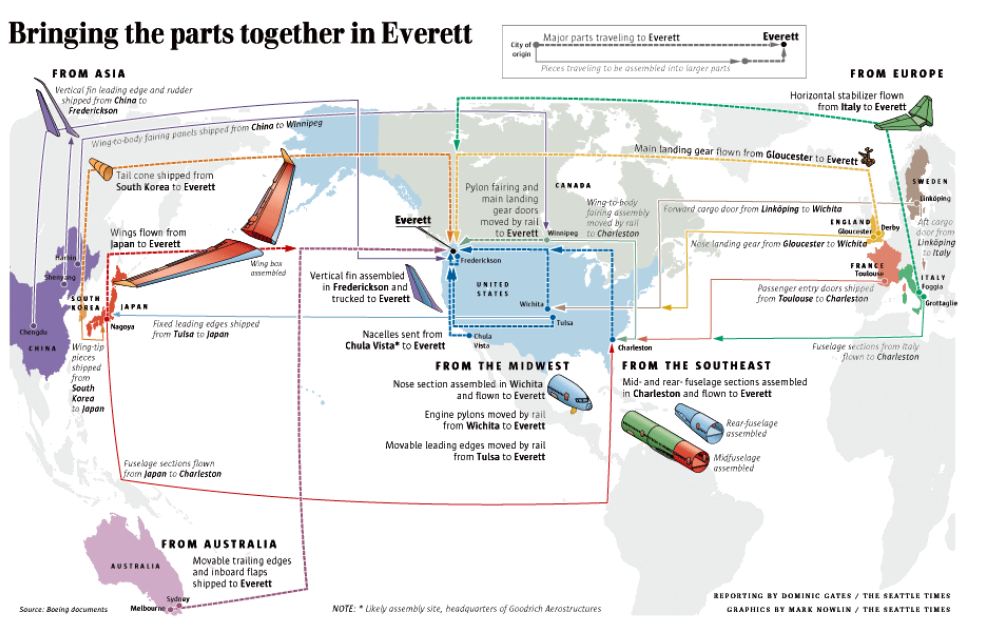
\includegraphics[width=0.8\textwidth]{boeing.jpg}
    \caption{Boeing 787 outsourced 70\% of its parts.}
  \end{figure}
\end{frame}

\begin{frame}{2015 Ukraine Power Outage}
  \begin{figure}[<+htpb+>]
    \begin{center}
      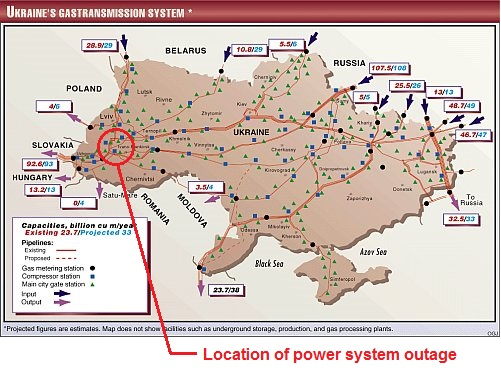
\includegraphics[width=0.60\textwidth]{ukraine.jpg}
      \caption{A successful attack on CPS can have devastating effects.}
    \end{center}
  \end{figure}
\end{frame}

\begin{frame}{What is New in CPS Security?}
  Why not just use information security?
  \begin{enumerate}
  \item Physics
  \item Physical Attacks: GPS Spoofing, etc.
  \item Zero-day Attacks: Attack that exploits undiscovered vulnerabilities.
  \item Cost: Securing every single device is difficult and costly
  \item High reliability requirement
  \end{enumerate}
\end{frame}

\begin{frame}{Defense in Depth}
  \begin{figure}[<+htpb+>]
    \begin{center}
      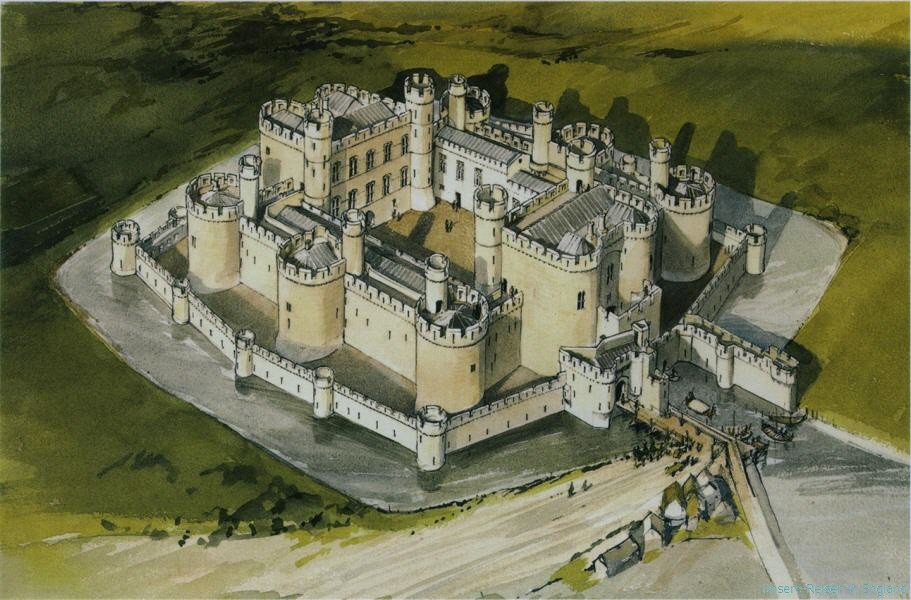
\includegraphics[width=0.8\textwidth]{defense_in_depth.jpg}
      \caption{Combining System Theory and Information Security to create better Protection for CPS}
    \end{center}
  \end{figure}
\end{frame}

\begin{frame}{Hardening CPS Security using System Theory}
  \begin{itemize}
  \item System and Attack Modelling
  \item Intrusion Detection and Isolation
  \item Resilient Algorithm Design
  \item Fundamental Limitations
  \item Security System Design and Investment
  \item \dots
  \end{itemize}
\end{frame}

\frame{\tableofcontents}

\section{Hypothesis Testing}

\begin{frame}{A Classical Hypothesis Testing Problem}
  \begin{itemize}
  \item We want to decide whether a binary state $\theta$ is $0$ or $1$.
  \item $m$ identical sensors are measuring the state: 
  \begin{center}
    \setlength{\figureheight}{3cm}
    \setlength{\figurewidth}{10cm}
    \inputtikz{gaussian}
  \end{center}
  \item Let us define 
    \begin{displaymath}
      z(k) = \begin{bmatrix}z_1(k)&\dots&z_m(k)\end{bmatrix},\,Z(k) = \begin{bmatrix}z(1)&\dots&z(k)\end{bmatrix}.
    \end{displaymath}
  \item A detection strategy is an infinite sequence of detectors $f = (f_1,\,f_2,\,\dots)$, where each $f_k$ maps $Z(k)$ into a decison $\hat \theta(k)$.
  \end{itemize}
\end{frame}

\begin{frame}{A Classical Hypothesis Testing Problem}
 \begin{itemize}
  \item Without the attacker, the optimal detector is a Naive Bayes Detector:
    \begin{align*}
      \hat \theta(k)=f_k(Z(k))=\begin{cases}
        -1 &\text{if }\sum_{i=1}^m\sum_{t=1}^k z_i(t)/mk < 0\\
        +1 &\text{if }\sum_{i=1}^m\sum_{t=1}^k z_i(t)/mk \geq 0\\
      \end{cases}.
    \end{align*}
  \item However, it is not secure. 
  \end{itemize}   
\end{frame}

\begin{frame}{Byzantine Attack}
  \begin{itemize}
  \item The attacker can compromised $p$ sensors, the set of which is denoted as $\mathcal I$. 
    \begin{displaymath}
      y(k) = z(k) + a(k),  
    \end{displaymath}
    where $a_i(k) = 0$ if $i\notin \mathcal I$.
    \begin{center}
      \setlength{\figureheight}{2cm}
      \setlength{\figurewidth}{10cm}
      \inputtikz{blockdiagram}
    \end{center}
  \item The disturbance $a(k)$ depends $ Z(k)$ and $\mathcal I$: 
    \begin{displaymath}
      a(k) = g_k( Z(k),\mathcal I). 
    \end{displaymath}
  \item The attack strategy $g = (g_1,\,g_2,\,\dots)$.
  \item Assume that $p$ is less than half of $m$.
  \item The detector knows $p$, but does not know $\mathcal I$.
  \end{itemize}
\end{frame}

\begin{frame}{Performance: Probability of Error}
  \begin{itemize}
  \item The probability of error at time $k$ is denoted as
    \begin{displaymath}
      P_e(k) = \max_{\mathcal I,\theta}\; P(f_k(Y(k)) \neq \theta). 
    \end{displaymath}
  \item Clearly, $P_e(k)$ is a function of the detection strategy $f$ and the attack strategy $g$.
  \item  In general, for a fixed $k$, optimizing $P_e(k)$ directly (either from the system's perspective or the attacker's perspective) is difficult.
  \item As a result, we will focus on the asymptotic performance when $k\rightarrow\infty$.
  \end{itemize}
\end{frame}

\begin{frame}{Chernoff Information}
  \begin{itemize}
  \item Suppose we have a single benign sensor, the Naive Bayes Detector takes the following form:
    \begin{align*}
      \hat \theta(k)=f_k(Z(k))=\begin{cases}
        -1 &\text{if }\sum_{t=1}^k z_1(t)/k < 0\\
        +1 &\text{if }\sum_{t=1}^k z_1(t)/k \geq 0\\
      \end{cases}.
    \end{align*}
  \item By LLN, the probability of error goes to $0$.
  \item Moreover, it goes to $0$ exponentially fast, i.e.,
    \begin{displaymath}
      \lim_{k\rightarrow\infty}-\frac{\log P_e(k)}{k}= \frac{1}{2}.
    \end{displaymath}
  \item For multiple benign sensors, the probability of error for the Naive Bayes Detector satisfies:
    \begin{displaymath}
      P_e(k)\approx e^{-\frac{1}{2}mk}.
    \end{displaymath}
  \item For general pair of distributions, one can prove that $P_e \approx e^{-mCk}$, where $C$ is the Chernoff information between the two distributions.
  \end{itemize}
\end{frame}

\begin{frame}{Asymptotic Performance}
  \begin{itemize}
  \item In adversarial environment, let us define the rate function $I$ as
    \begin{displaymath}
      I = \liminf_{k\rightarrow\infty} -\frac{\log P_e(k)}{k}.
    \end{displaymath}
    Roughly speaking, 
    \begin{displaymath}
      P_e(k)\sim e^{-Ik}. 
    \end{displaymath}
    Larger rate implies better detection performance.
  \item  $I$ is a function of both detection strategy $f$ and attack strategy $g$.
  \item The detector wants to maximize $I$ while the attacker wants to minimize $I$.
  \item Question: Does there exist a pair of equilibrium strategy $(f^*,g^*)$, such that
    \begin{displaymath}
      I(f^*,g)\geq I(f^*,g^*) \geq I(f,g^*).	
    \end{displaymath}
  \end{itemize}
\end{frame}

\begin{frame}{``Optimal'' Attack Strategy $g^*$}
  \begin{itemize}
  \item Consider the attack, where the adversary simply flips the distribution of $p$ compromised sensors' measurements
    \begin{center}
      \inputtikz{attack}
    \end{center}
  \item The first $2p$ sensors have identical distribution.
  \item The only way to distinguish the two cases is to use the remaining $m-2p$ sensors.
  \item No detector can achieve a performance better than $(m-2p)C$ (Even if they know the adversary's strategy).
  \end{itemize}
\end{frame}

\begin{frame}{``Optimal'' Detection Strategy $f^*$}
  We need to define the following trimmed sum functions:
  \begin{definition}
    Define the symmetric functions $\Smin_{2p},\,\Smid_{2p},\,\Smax_{2p}:\mathbb R^{m}\rightarrow \mathbb R$ as  
    \begin{align*}
      \Smin_{2p}(y_1,\ldots,y_m) &\triangleq \sum_{i=1}^{m-2p}y_i,\\
      \Smid_{2p}(y_1,\ldots,y_m) &\triangleq \sum_{i=p+1}^{m-p}y_i,\\
      \Smax_{2p}(y_1,\ldots,y_m) &\triangleq \sum_{i=2p+1}^{m}y_i,
    \end{align*}
    when $y_1\leq \dots\leq y_m$.
  \end{definition}
\end{frame}

\begin{frame}{``Optimal'' Detection Strategy $f^*$}
  \begin{itemize}
  \item If $\|y - z\|_0\leq p$, then
    \begin{displaymath}
      \Smin_{2p}(z) \leq \Smid_{2p}(y)\leq \Smax_{2p}(z).
    \end{displaymath} 
  \item Assuming $m=5$, $p = 1$:
    \begin{center}
      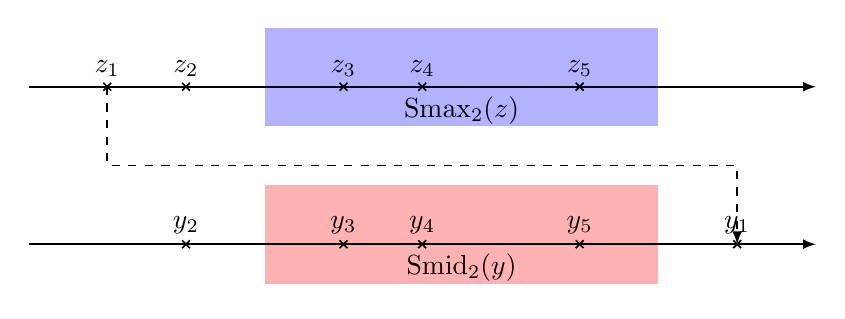
\begin{tikzpicture}[semithick,>=latex]
        \draw [->] (0,0)--(10,0);
        \draw plot[mark=x] coordinates{(1,0)} node [above] {$z_1$};
        \draw plot[mark=x] coordinates{(2,0)} node [above] {$z_2$};
        \draw plot[mark=x] coordinates{(4,0)} node [above] {$z_3$};
        \draw plot[mark=x] coordinates{(5,0)} node [above] {$z_4$};
        \draw plot[mark=x] coordinates{(7,0)} node [above] {$z_5$};
        
        \draw [->] (0,-2)--(10,-2);
        \draw plot[mark=x] coordinates{(9,-2)} node [above] {$y_1$};
        \draw plot[mark=x] coordinates{(2,-2)} node [above] {$y_2$};
        \draw plot[mark=x] coordinates{(4,-2)} node [above] {$y_3$};
        \draw plot[mark=x] coordinates{(5,-2)} node [above] {$y_4$};
        \draw plot[mark=x] coordinates{(7,-2)} node [above] {$y_5$};
        
        \draw [->,dashed] (1,0)--(1,-1)--(9,-1)--(9,-2);
        \begin{pgfonlayer}{background}
          \fill [fill=red!30] (3,-2.5) rectangle (8,-1.25);
          \node at (5.5,-2.3) {$\Smid_2(y)$};
          
          \fill [fill=blue!30] (3,-0.5) rectangle (8,0.75);
          \node at (5.5,-0.3) {$\Smax_2(z)$};
        \end{pgfonlayer}
      \end{tikzpicture}
    \end{center}
  \item $\Smid_{2p}$ is a more ``secure'' version of sum. 
  \item $\Smid_{2p}(y) < 0$ as long as $\Smax_{2p}(z)< 0$..
  \end{itemize}
\end{frame}

\begin{frame}{Equilibrium Strategies}
  \it Theorem: The following strategy pair $(f^*,g^*)$ forms a Nash-equilibrium with $I(f^*,g^*) = (m-2p)C$:
  \begin{block}{Attack Strategy $g^*$}
    Flip $p$ compromised sensors' measurements.
  \end{block}
  \begin{block}{Detection Strategy $f^*$}
    \begin{enumerate}
    \item For each sensor $i$, compute a local average $ \bar y_i(k) = \sum_{t=1}^k y_i(t)$.
    \item The detector $f_k$ is given by
      \begin{displaymath}
        f_k(Y(k)) = \begin{cases}
          -1 &\text{if }\Smid_{2p}(\bar y(k))< 0\\
          1 &\text{if }\Smid_{2p}(\bar y(k))\geq 0\\
        \end{cases}
      \end{displaymath}
    \end{enumerate}
  \end{block}
\end{frame}

\begin{frame}{What is the Cost of Security?}
  \begin{itemize}
  \item We need to consider the system performance both in the presence and in the absence of the attack.
    \vspace{0.5cm}
    \begin{center}
      \inputtikz{fun_lim2}
    \end{center}
  \item Unfortunately, trimmed sum has an efficiency of $(m-p)C$.
  \item How to get perfect security and efficiency simultaneously?
  \end{itemize}
\end{frame}

\begin{frame}{Cost-Free Security}
  For Gaussian case, there exists algorithm achieving perfect security and efficiency simultaneously.
  \begin{enumerate}
  \item If there exists a set $J$ of $m-p$ sensors, such that
    \begin{align*}
      \sum_{i\in \mathcal J}\frac{1}{2}(\bar y_i+1)^2 < (m-2p)C,
    \end{align*}
    then choose $\hat \theta = 0$. 
  \item If there exists a set $J$ of $m-p$ sensors, such that
    \begin{align*}
      \sum_{i\in \mathcal J}\frac{1}{2}(\bar y_i-1)^2 < (m-2p)C,
    \end{align*}
    then choose $\hat \theta = 1$. 
  \item If none of the above conditions are satisfied, do a Naive Bayes test.
  \end{enumerate}
\end{frame}

\begin{frame}{Cost-Free Security}
  \begin{itemize}
  \item The best security $(m-2n)C$ and the best efficiency $mC$ are achieved simultaneously
  \item Security is ``cost-free''
    \begin{itemize}
    \item Computational burden: $O(m)$ versus $O(m\log m)$
    \end{itemize}
  \item Generalization: ``symmetric'' distributions. There exists a constant $a$ such that 
    \begin{align*}
      p_0(a+z) = p_1(a-z).
    \end{align*}
  \end{itemize}
\end{frame}

\begin{frame}{Generalization: Unknown Number of Compromised sensors}
  \begin{enumerate}
  \item Set $p = \lfloor m/2\rfloor -1$.
  \item 
    \begin{itemize}
    \item If there exists a set $J$ of $m-p$ sensors, such that
      \begin{align*}
        \sum_{i\in \mathcal J}\frac{1}{2}(\bar y_i+1)^2 < (m-2p)C,
      \end{align*}
      then choose $\hat \theta = 0$. 
    \item If there exists a set $J$ of $m-p$ sensors, such that
      \begin{align*}
        \sum_{i\in \mathcal J}\frac{1}{2}(\bar y_i-1)^2 < (m-2p)C,
      \end{align*}
      then choose $\hat \theta = 1$. 
    \end{itemize}
  \item Reduce $p$ by 1. If $p > 0$, go back to step 2, otherwise do a Naive Bayes test.
  \end{enumerate}
  The above algorithm is optimal for any number of compromised sensors.
\end{frame}

\begin{frame}{General Case: Some Definitions from Large Deviation Theory}
  \begin{center}
    \inputtikz{rate_function}
  \end{center}
  \begin{itemize}
  \item $I_\theta(y) \triangleq \sup_{w} yw - \log \mathbb E_\theta exp(\lambda w).$
  \item $I_\theta(y)$ measures how typical a measurement $y$ is under each hypothesis.
  \end{itemize}
\end{frame}

\begin{frame}{General Cases}
  \begin{center}
    \inputtikz{fun_lim}
  \end{center}
  Fundamental Trade-off:
  \begin{align*}
I_0^{-1}\left(\frac{s}{m-n}\right)\leq I_1^{-1}\left(\frac{e}{m-n}\right),\, I_0^{-1}\left(\frac{e}{m-n}\right)\leq I_1^{-1}\left(\frac{s}{m-n}\right). 
  \end{align*}
  For the Gaussian case, the blue and red line will not cut the corner.
\end{frame}

\begin{frame}{General Case}
  The following detection strategy achieves the fundamental limit:
  \begin{enumerate}
  \item If there exists a set $J$ of $m-p$ sensors, such that
    \begin{align*}
      \sum_{i\in \mathcal J}I_0(\bar \lambda_i) < threshold,
    \end{align*}
    then choose $\hat \theta = 0$. 
  \item If there exists a set $J$ of $m-p$ sensors, such that
    \begin{align*}
      \sum_{i\in \mathcal J}I_1(\bar \lambda_i) < threshold,
    \end{align*}
    then choose $\hat \theta = 1$. 
  \item If none of the above conditions are satisfied, do a Naive Bayes test.
  \end{enumerate}
\end{frame}

\begin{frame}{Simulation}
  Assuming the following distribution:
  \begin{center}
    \begin{tabular}{@{}llr@{}}
      \toprule
      & $z = 0$ & $z=1$\\
      \midrule
      $\theta=0$ &0.98&0.02\\
      $\theta=1$ &0.4&0.6\\
      \bottomrule
    \end{tabular}
  \end{center}  
  We choose the detector with perfect efficiency:
  \begin{center}
    \inputtikz{finite_time}
  \end{center}
\end{frame}

\section{State Estimation}

\begin{frame}{Static State Estimation}
  \begin{enumerate}
  \item We assume that $x \in \mathbb R^n$ is the state that we want to estimate.
  \item $m$ sensors are deployed to monitor the system. Denote $z_i \in \mathbb R$ as the measurement generated by sensor $i$.
  \item Denote $z = \begin{bmatrix}z_1&\dots&z_m\end{bmatrix}^T$ as the collection of all sensory data.
  \item We assume the following sensor model:
    \begin{align*}
      z = Hx + w,
    \end{align*}
    where $H$ is a matrix of proper dimension and $w$ represent random noise.
  \item The optimal state estimator is of the form
    \begin{align*}
      \hat x = Kz, \text{ where }K = (H^TH)^{-1}H^T.
    \end{align*}
  \end{enumerate}
\end{frame}

\begin{frame}{Least Square Estimator}
  Suppose the following sensory model:
  \begin{align*}
    y = \begin{bmatrix}
      1\\
      1\\
      1
    \end{bmatrix}x + w.
  \end{align*}
  The optimal estimator is given by
  \begin{align*}
    \hat x = \frac{1}{3}\left(y_1+y_2+y_3\right).
  \end{align*}
  
  This estimator is not resilient to a single malicious sensor.
\end{frame}

\begin{frame}{Problem Formulation}
  \begin{enumerate}
  \item Assume that at most $p$ sensors are compromised.
  \item The sensory model is given by
    \begin{align*}
      y = z + a = Hx + w +a,
    \end{align*}
    where $a$ is a $p$-sparse vector indicating the attacker's action.
  \item We will call an estimator $\hat x = g(y)$ to be resilient if
    \begin{align*}
      \|g(y) - g(z)\|\text{ is bounded for all $p$-sparse $a$}.
    \end{align*}
  \item The total state estimation error can be written as
    \begin{align*}
      x-g(y) = x-g(z) + g(z)-g(y).
    \end{align*}

  \end{enumerate}
\end{frame}

\begin{frame}{Why not use bad data detection?}
  \begin{center}

    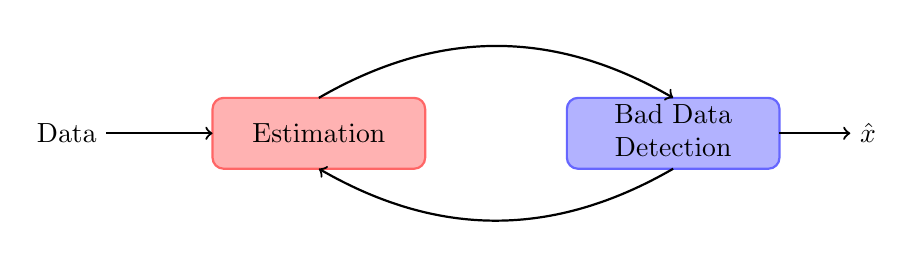
\begin{tikzpicture}[scale=0.9]
      \draw[thick,rounded corners,fill=red!30,draw=red!60] (0,1) rectangle (3,2);
      \node at (1.5,1.5) {Estimation};

      \draw[thick,rounded corners,fill=blue!30,draw=blue!60] (5,1) rectangle (8,2);
      \node at (6.5,1.5) {\begin{tabular}{c} Bad Data\\ Detection \end{tabular}};

      \draw[thick,->] (-1.5,1.5)--(0,1.5);
      \node [anchor=east] at (-1.5,1.5) {Data};

      % \draw[thick,->] (3,1.5) to (5,1.5);

      \draw[thick,->] (1.5,2) to [bend left] (6.5,2);
      \draw[thick,->] (6.5,1) to [bend left] (1.5,1);

      \draw[thick,->] (8,1.5) to (9,1.5);

      \node [anchor=west] at (9,1.5) {$\hat x$};
    \end{tikzpicture}
  \end{center}
  \begin{enumerate}
  \item A typical bad data detector will first compute $\hat x = Ky$ and then the residue $r = y - H\hat x$.
  \item The bad data detector will then remove the sensors with large residue.
  \item Drawbacks: It is designed for \emph{random failures}, not necessarily attacks; Difficult to analyze the estimation performance.
  \end{enumerate}
\end{frame}

\begin{frame}{Some Related Research}
  \begin{enumerate}
  \item The following estimator is resilient under $2p$ observable condition:
    \begin{align*}
      & \mathop{\textit{minimize}}\limits_{\hat x,a,w}&
      & \|w\|^2 \\
      &\text{subject to}&
      &y = H \hat x + w + a,\,\|a\|_0\leq p.
    \end{align*}
    The drawback: The optimization problem is not convex and solving it is computationally difficult.
  \item We can use convex optimization based estimator, e.g., 
    \begin{align*}
      & \mathop{\textit{minimize}}\limits_{\hat x,a,w}&
      & \|w\|^2 + \|a\|_1 \\
      &\text{subject to}&
      &y = H \hat x + w + a.
    \end{align*}
    However, there is no direct proof on its resiliency.
  \item What about other type of estimators?
  \end{enumerate}
\end{frame}

\begin{frame}{A General Convex Optimization Based Estimator}
  We consider the following estimator
  \begin{align*}
    \hat x = g(y) \triangleq \argmin_{\hat x} \sum_{i=1}^m f_i(y_i-H_i \hat x),
  \end{align*}
  where the following properties of function $f_i:\mathbb R\mapsto \mathbb R$ are assumed:
  \begin{enumerate}
  \item $f_i$ is convex.
  \item $f_i$ is symmetric, i.e., $f_i(u) = f_i(-u)$.
  \item $f_i$ is non-negative and $f_i(0) = 0$.
  \end{enumerate} 

  If we define the residue $r_i\triangleq y_i - H_i\hat x$, then we are trying to minimize the sum of some cost function related to the residue.

  The estimator can be computed efficiently via convex optimization. 
\end{frame}


\begin{frame}{A General Convex Optimization Based Estimator}
  Our proposed estimator is very general since we can choose the right $f_i$ to get the following estimator:
  \begin{enumerate}
  \item Linear Estimator:
    \begin{align*}
      g(y) = \argmin_{\hat x} \|y-H\hat x\|_2^2= \argmin_{\hat x}  \sum_{i=1}^m (y_i-H_i\hat x)^2.
    \end{align*}
  \item $L_1$ Estimator:
    \begin{align*}
      g(y) = \argmin_{\hat x} \|y-H\hat x\|_1=\argmin_{\hat x} \sum_{i=1}^m |y_i-H_i\hat x|.
    \end{align*}
  \end{enumerate}
\end{frame}

\begin{frame}{A General Convex Optimization Based Estimator}
  \begin{enumerate}  \setcounter{enumi}{2}
  \item LASSO:
    \begin{align*}
      g(y) = \argmin_{\hat x} \|w\|^2+\lambda \|a\|_1, \text{ s.t. }y=H\hat x+w+a.
    \end{align*}
    After some manipulations, we can rewrite the optimization problem as
    \begin{align*}
      g(y) = \argmin_{\hat x} \sum_{i=1}^m f(y_i-H_i\hat x)
    \end{align*}
    where
    \begin{align*}
      f(r) = \min_{w} w^2 + \lambda |r-w| = \begin{cases}
        r^2 & \text{if } r \leq \lambda/2\\
        \lambda |r|-\lambda^2/4 & \text{if } r\geq \lambda/2\\
      \end{cases}.
    \end{align*}
  \end{enumerate}
\end{frame}

\begin{frame}{Example}
  Suppose the following sensory model:
  \begin{align*}
    y = \begin{bmatrix}
      1\\
      1\\
      1
    \end{bmatrix}x + w+a,\,\|a\|_0\leq 1.
  \end{align*}
  Then the following estimator is resilient (in fact, it is the median of $y_i$):
  \begin{align*}
    g(y) = \argmin_{\hat x}  |y_1-\hat x|+|y_2-\hat x|+|y_3-\hat x|.
  \end{align*}
\end{frame}

\begin{frame}{Example}
  \begin{figure}[ht]
    \centering
    \begin{tikzpicture}[yscale=0.4]
      \draw[thick,->] (0,0)--(9,0);
      \node [anchor=west] at (9,0) {$\hat x$};
      \draw[thin,gray] (2,0)--(2,0.1);
      \draw[thin,gray] (5,0)--(5,0.1);
      \draw[thin,gray] (7,0)--(7,0.1);
      \draw[thick](1,11)--(2,8)--(5,5)--(7,7)--(8,10);
      \node [anchor=north] at (2,0) {\color{red}{$y_1$}};
      \node [anchor=north] at (5,0) {\color{blue}{$y_2$}};
      \node [anchor=north] at (7,0) {\color{brown}{$y_3$}};
    \end{tikzpicture}
  \end{figure}
  \color{white}{If we interpret the function $|y_i-\hat x|$ as a potential function generate by sensor $i$, then we can see that sensor $i$ is dragging $\hat x$ towards $y_i$ with $1$ unit of force. The equilibrium point will be at the middle $y_i$.}
\end{frame}

\begin{frame}{Interpretation}
  \begin{figure}[ht]
    \centering
    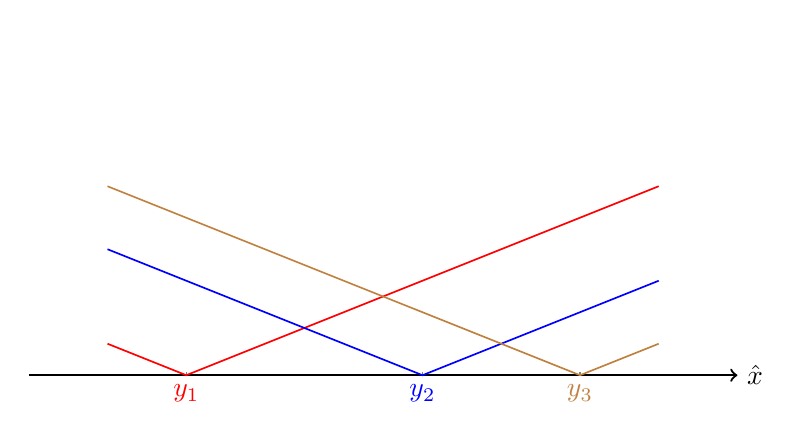
\begin{tikzpicture}[yscale=0.4]
      \draw[thick,->] (0,0)--(9,0);
      \node [anchor=west] at (9,0) {$\hat x$};
      \draw[thin,gray] (2,0)--(2,0.1);
      \draw[thin,gray] (5,0)--(5,0.1);
      \draw[thin,gray] (7,0)--(7,0.1);
      \draw[thick,white](1,11)--(2,8)--(5,5)--(7,7)--(8,10);
      \node [anchor=north] at (2,0) {\color{red}{$y_1$}};
      \draw[semithick,red](1,1)--(2,0)--(8,6);
      \node [anchor=north] at (5,0) {\color{blue}{$y_2$}};
      \draw[semithick,blue](1,4)--(5,0)--(8,3);
      \node [anchor=north] at (7,0) {\color{brown}{$y_3$}};
      \draw[semithick,brown](1,6)--(7,0)--(8,1);
    \end{tikzpicture}
  \end{figure}
  If we interpret the function $|y_i-\hat x|$ as a potential function generate by sensor $i$, then we can see that sensor $i$ is dragging $\hat x$ towards $y_i$ with $1$ unit of force. The equilibrium point will be at the middle $y_i$.
\end{frame}

\begin{frame}{Another Example}
  Suppose the following sensory model:
  \begin{align*}
    y = \begin{bmatrix}
      1\\
      1\\
      3
    \end{bmatrix}x + w+a ,\,\|a\|_0\leq 1.
  \end{align*}
  Then the following estimator is not resilient:
  \begin{align*}
    g(y) = \argmin_{\hat x}  |y_1-\hat x|+|y_2-\hat x|+|y_3-3\hat x|.
  \end{align*}
  In fact, we can rewrite it as
  \begin{align*}
    g(y) = \argmin_{\hat x}  |y_1-\hat x|+|y_2-\hat x|+3\left|\frac{y_3}{3}-\hat x\right| = \frac{y_3}{3}
  \end{align*}
  Sensor $3$ generates $3$ unit of force comparing to $1$ unit of force from sensor $1$ and $2$.
\end{frame}

\begin{frame}{Sufficient Condition For Resiliency}
  \begin{theorem}
    If the following conditions hold, then the estimation is resilient:
    \begin{enumerate}
    \item For all $i$, the following limit is well-defined:
      \begin{align*}
        \lim_{t\rightarrow\infty}\frac{f_i(t)}{t} = \alpha_i < \infty.
      \end{align*}
    \item For any $u\neq 0$ and any index set $\mathcal I$ of cardinality $p$, the following inequality hold:
      \begin{align*}
        \sum_{i\in \mathcal I} |\alpha_i H_i u| < \sum_{i\in \mathcal I^c} |\alpha_i H_i u|.
      \end{align*}
    \end{enumerate}
  \end{theorem}
  Roughly speaking $|\alpha_i H_i u|$ is the maximum force from sensor $i$. The condition can be interpreted as the combined force from any $p$ sensors should be smaller than that of the remaining $m-p$ sensors.
\end{frame}

\begin{frame}{Necessary Condition For Resiliency}
  \begin{theorem}
    If the one of the following conditions is violated, then the estimation is not resilient:
    \begin{enumerate}
    \item There exists an $i$, such that
      \begin{align*}
        \lim_{t\rightarrow\infty}\frac{f_i(t)}{t} = \infty.
      \end{align*}
    \item There exists a $u\neq 0$ and an index set $\mathcal I$ of cardinality $p$, such that
      \begin{align*}
        \sum_{i\in \mathcal I} |\alpha_i H_i u| > \sum_{i=\mathcal I^c} |\alpha_i H_i u|.
      \end{align*}
    \end{enumerate}
  \end{theorem}
  Notice that we only have a trivial gap for the case:
  \[ \sum_{i\in \mathcal I} |\alpha_i H_i u| = \sum_{i=\mathcal I^c} |\alpha_i H_i u|.\]
\end{frame}

\begin{frame}{How to Handle Correlated Noise}
  Instead of the problem where the residues are decoupled:
  \begin{align*}
    g(y) = \argmin_{\hat x} \sum_{i=1}^m f_i(r_i),\text{s.t.}y_i = H_i\hat x+r_i,
  \end{align*}
  we could also consider the estimator where part of the residue are coupled via a quadratic term:
  \begin{align*}
    g(y) = \argmin_{\hat x}  w^TQw+\sum_{i=1}^m f_i(a_i),\text{s.t.}y_i = H_i\hat x+w_i+a_i.
  \end{align*}
  The sufficient condition for resiliency remains the same.
\end{frame}

\begin{frame}{Simulation IEEE 14-bus System}
  \begin{figure}[ht]
    \centering
    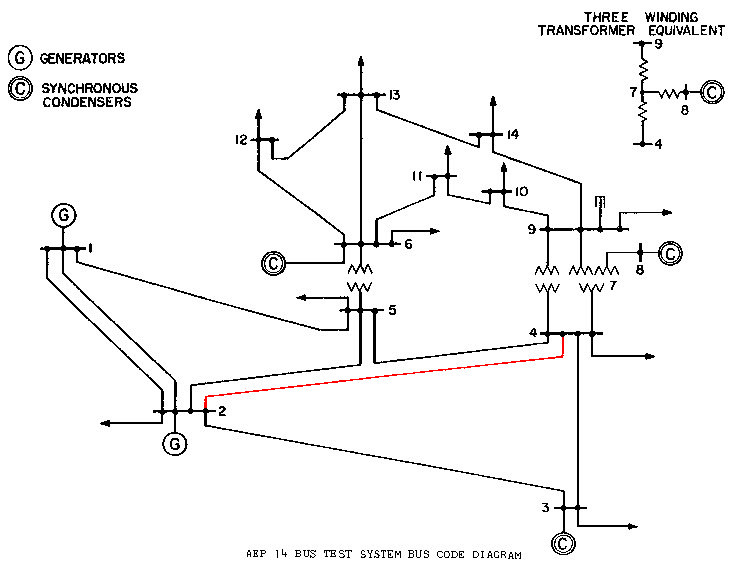
\includegraphics[width=0.60\textwidth]{ieee14.jpg}
  \end{figure}
  We assume $p=1$ and the flow sensor on the red line is being attacked.
\end{frame}

\begin{frame}{Simulation IEEE 14-bus System}
  \begin{figure}[ht]
    \begin{center}
      
      \setlength{\figureheight}{6cm}
      \setlength{\figurewidth}{10cm}
      \definecolor{mycolor1}{rgb}{1.00000,0.00000,1.00000}%
      % 
      \begin{tikzpicture}

        \begin{axis}[%
          width=\figurewidth,
          height=\figureheight,
          at={(1.527in,1.083in)},
          scale only axis,
          xmin=0.95,
          xmax=2.4,
          xlabel={Normalized MSE of the estimators without attack},
          xmajorgrids,
          ymin=0.95,
          ymax=2.5,
          ylabel={Normalized MSE when under attack},
          ymajorgrids,
          axis background/.style={fill=white},
          legend style={at={(0.597,0.528)},anchor=south west,legend cell align=left,align=left,draw=white!15!black}
          ]
          \addplot [color=blue,dashed,line width=1.5pt,mark=triangle,mark options={solid},forget plot]
          table[row sep=crcr]{%
            2.16434829886514	2.41673714136766\\
            1.49824142620916	1.6273922047888\\
            1.46836558726546	1.61304395019434\\
            1.42878218405531	1.58080265845186\\
            1.33509034059386	1.48317348510781\\
            1.24979953097586	1.4011442907391\\
            1.20190884155895	1.36475282176979\\
            1.14816845697376	1.32743887772808\\
            1.104692902235	1.30458587111275\\
            1.0727554366346	1.2930587844785\\
            1.04837293442887	1.29286647088633\\
            1.03276380632143	1.30464750437787\\
            1.02491383863213	1.32636243694814\\
            1.0209295289153	1.35606289076979\\
            1.01470702949196	1.40680155569416\\
            1.00686189169388	1.48274325705327\\
            1.00166658882151	1.69020329692052\\
            1.00012894457222	2.29806950301701\\
          };

          \addplot [color=mycolor1,dashed,forget plot]
          table[row sep=crcr]{%
            1	1\\
            2.2	1\\
          };
          \addplot [color=mycolor1,dashed,forget plot]
          table[row sep=crcr]{%
            1	1\\
            1	2.5\\
          };
          \node[right, align=left, text=blue]
          at (axis cs:2.164,2.417) {$\text{   }\leftarrow\text{ }\lambda\rightarrow 0$};
          \node[right, align=left, text=blue]
          at (axis cs:1.335,1.483) {$\text{   }\leftarrow\text{ }\lambda\text{=0.5}$};
          \node[right, align=left, text=blue]
          at (axis cs:1.202,1.365) {$\text{   }\leftarrow\text{ }\lambda\text{=1}$};
          \node[right, align=left, text=blue]
          at (axis cs:1.073,1.293) {$\text{   }\leftarrow\text{ }\lambda\text{=1.9}$};
          \node[right, align=left, text=blue]
          at (axis cs:1.02,1.356) {$\leftarrow\lambda\text{=3}$};
          \node[right, align=left, text=blue]
          at (axis cs:1,2.298) {$\text{   }\leftarrow\text{ }\lambda\text{=7}$};
          \node[right, align=left, text=mycolor1]
          at (axis cs:1,2.4) {$\text{   }\leftarrow\text{ LSE}$};
          \node[right, align=left, text=mycolor1]
          at (axis cs:1.9,1.14) {Oracle LSE};
          \node[right, align=left, text=mycolor1]
          at (axis cs:1.9,1.07) {$\text{     ~~~~~}\downarrow$};
        \end{axis}
      \end{tikzpicture}%
    \end{center}
  \end{figure}
\end{frame}

\begin{frame}{Dynamic State Estimation}
  \begin{enumerate}
  \item Consider the following dynamic system
    \begin{align}
      x(k+1) = A x(k) + w(k),\, y(k) = C x(k) + v(k) + a(k).
    \end{align}
  \item A linear fixed-gain estimator:
    \begin{align}
      \hat x(k+1) = A \hat x(k) + K(y(k+1)-CA\hat x(k)),
    \end{align}
    where $K$ is the estimation gain, and $A-KCA$ is stable.
    \begin{center}
      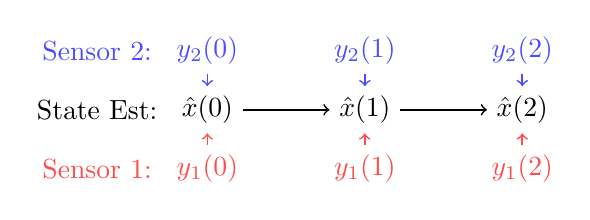
\begin{tikzpicture}[x=2cm, y=0.75cm]
        \node at (-0.7,0) {State Est:};
        \node [blue!70] at (-0.7,1) {Sensor 2:};
        \node [red!70] at (-0.7,-1) {Sensor 1:};

        \node            (x0)  at (0,0) {$\hat x(0)$};
        \node [blue!70] (y20)  at (0,1)    {$y_2(0)$};
        \node [red!70]  (y10)  at (0,-1)   {$y_1(0)$};
        \draw [->,semithick,blue!70] (y20) to (x0);
        \draw [->,semithick,red!70]  (y10) to (x0);

        \node            (x1)  at (1,0) {$\hat x(1)$};
        \node [blue!70] (y21)  at (1,1)    {$y_2(1)$};
        \node [red!70]  (y11)  at (1,-1)   {$y_1(1)$};
        \draw [->,semithick,blue!70] (y21) to (x1);
        \draw [->,semithick,red!70]  (y11) to (x1);

        \node            (x2)  at (2,0) {$\hat x(2)$};
        \node [blue!70] (y22)  at (2,1)    {$y_2(2)$};
        \node [red!70]  (y12)  at (2,-1)   {$y_1(2)$};
        \draw [->,semithick,blue!70] (y22) to (x2);
        \draw [->,semithick,red!70]  (y12) to (x2);

        \draw [->,semithick] (x0) to (x1);
        \draw [->,semithick] (x1) to (x2);
      \end{tikzpicture}
    \end{center}
  \item The error introduced by the attack may accumulate over time.
  \end{enumerate}
\end{frame}

\begin{frame}{Dynamic State Estimate: A Moving Horizon Approach}
  In order to convert the dynamic estimation problem into a static one, we can use a moving horizon approach:
  \begin{center}
    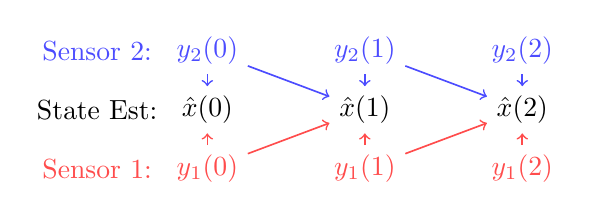
\begin{tikzpicture}[x=2cm, y=0.75cm]
      \node at (-0.7,0) {State Est:};
      \node [blue!70] at (-0.7,1) {Sensor 2:};
      \node [red!70] at (-0.7,-1) {Sensor 1:};

      \node            (x0)  at (0,0) {$\hat x(0)$};
      \node [blue!70] (y20)  at (0,1)    {$y_2(0)$};
      \node [red!70]  (y10)  at (0,-1)   {$y_1(0)$};
      \draw [->,semithick,blue!70] (y20) to (x0);
      \draw [->,semithick,red!70]  (y10) to (x0);

      \node            (x1)  at (1,0) {$\hat x(1)$};
      \node [blue!70] (y21)  at (1,1)    {$y_2(1)$};
      \node [red!70]  (y11)  at (1,-1)   {$y_1(1)$};
      \draw [->,semithick,blue!70] (y21) to (x1);
      \draw [->,semithick,red!70]  (y11) to (x1);
      \draw [->,semithick,blue!70] (y20) to (x1);
      \draw [->,semithick,red!70]  (y10) to (x1);

      \node            (x2)  at (2,0) {$\hat x(2)$};
      \node [blue!70] (y22)  at (2,1)    {$y_2(2)$};
      \node [red!70]  (y12)  at (2,-1)   {$y_1(2)$};
      \draw [->,semithick,blue!70] (y22) to (x2);
      \draw [->,semithick,red!70]  (y12) to (x2);
      \draw [->,semithick,blue!70] (y21) to (x2);
      \draw [->,semithick,red!70]  (y11) to (x2);
    \end{tikzpicture}
  \end{center}

  However, the historical data are discarded and the estimation performance may be poor when the system is operating normally.
\end{frame}

\begin{frame}{Dynamic State Estimate: A Local Estimator Approach}
  We propose to store historical data in the local estimations:
  \begin{center}
    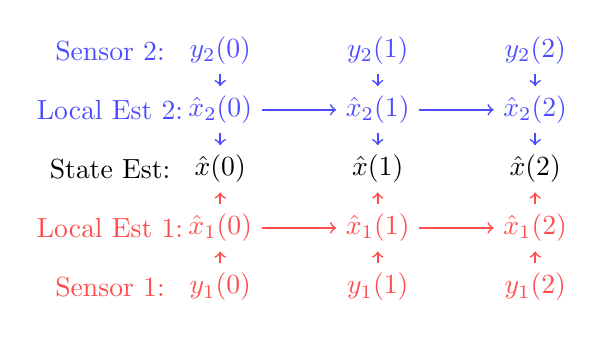
\begin{tikzpicture}[x=2cm, y=0.75cm]
      \node at (-0.7,0) {State Est:};
      \node [blue!70] at (-0.7,2) {Sensor 2:};
      \node [blue!70] at (-0.7,1) {Local Est 2:};
      \node [red!70] at (-0.7,-2) {Sensor 1:};
      \node [red!70] at (-0.7,-1) {Local Est 1:};

      \node            (x0)  at (0,0)    {$\hat x(0)$};
      \node [blue!70] (y20)  at (0,2)       {$y_2(0)$};
      \node [blue!70] (x20)  at (0,1)  {$\hat x_2(0)$};
      \node [red!70]  (y10)  at (0,-2)      {$y_1(0)$};
      \node [red!70]  (x10)  at (0,-1) {$\hat x_1(0)$};
      \draw [->,semithick,blue!70] (y20) to (x20);
      \draw [->,semithick,red!70]  (y10) to (x10);
      \draw [->,semithick,blue!70] (x20) to  (x0);
      \draw [->,semithick,red!70]  (x10) to  (x0);

      \node            (x1)  at (1,0)    {$\hat x(1)$};
      \node [blue!70] (y21)  at (1,2)       {$y_2(1)$};
      \node [blue!70] (x21)  at (1,1)  {$\hat x_2(1)$};
      \node [red!70]  (y11)  at (1,-2)      {$y_1(1)$};
      \node [red!70]  (x11)  at (1,-1) {$\hat x_1(1)$};
      \draw [->,semithick,blue!70] (y21) to (x21);
      \draw [->,semithick,red!70]  (y11) to (x11);
      \draw [->,semithick,blue!70] (x21) to  (x1);
      \draw [->,semithick,red!70]  (x11) to  (x1);

      \node            (x2)  at (2,0)    {$\hat x(2)$};
      \node [blue!70] (y22)  at (2,2)       {$y_2(2)$};
      \node [blue!70] (x22)  at (2,1)  {$\hat x_2(2)$};
      \node [red!70]  (y12)  at (2,-2)      {$y_1(2)$};
      \node [red!70]  (x12)  at (2,-1) {$\hat x_1(2)$};
      \draw [->,semithick,blue!70] (y22) to (x22);
      \draw [->,semithick,red!70]  (y12) to (x12);
      \draw [->,semithick,blue!70] (x22) to  (x2);
      \draw [->,semithick,red!70]  (x12) to  (x2);

      \draw [->,semithick,blue!70] (x20) to (x21);
      \draw [->,semithick,blue!70] (x21) to (x22);
      \draw [->,semithick,red!70] (x10) to (x11);
      \draw [->,semithick,red!70] (x11) to (x12);
    \end{tikzpicture}
  \end{center}
  \begin{enumerate}
  \item Construct local estimators (which uses only the local measurements):
    \begin{align*}
      \hat x_i(k) = A \hat x_i(k) + L_i (y_i(k)-CA\hat x_i(k)).
    \end{align*}  
  \item Reconstruct the global estimator as
    \begin{align*}
      \hat x(k) = g(\hat x_1(k),\ldots,\hat x_m(k)).
    \end{align*}  
  \end{enumerate}
\end{frame}

\begin{frame}{Local Estimator Design}
  \begin{enumerate}
  \item  Choose $L_i$ such that $A-L_iCA$ shares the same eigenvalues as $A-KCA$ (requires observability)
    \begin{align*}
      \hat x_i(k) = A \hat x_i(k) + L_i (y_i(k)-CA\hat x_i(k)).
    \end{align*}  
  \item The global estimate can be recovered as
    \begin{align*}
      \hat x(k) = F_1\hat x_1(k)+\dots+F_m\hat x_m(k).
    \end{align*}
  \item More importantly, it can be written as the solution of a quadratic programming problem:
    \begin{align*}
      &\mathop{\textrm{minimize}}\limits_{\hat x(k),\hat e(k)}&
      & \frac{1}{2}\hat e(k)^T \tilde W^{-1} \hat e(k)\\
      &\textrm{subject to} &
      &\hat x_i(k)  =  \hat x(k) + \hat e_i(k),&
    \end{align*}
  \end{enumerate}
\end{frame}

\begin{frame}{Securing the Global Estimate}
  We can secure the global estimator using LASSO:
  \begin{align*}
    &\mathop{\textrm{minimize}}\limits_{\hat x(k),\hat e(k)}&
    & \frac{1}{2}\hat e(k)^T \tilde W^{-1} \hat e(k) + \gamma \sum_{i=1}^m \|\hat \nu_i(k)\|_1\\
    &\textrm{subject to} &
    &\hat x_i(k)  =  \hat x(k) + \hat e_i(k)+\hat \nu_i(k),&
  \end{align*}
\end{frame}

\begin{frame}{Efficiency and Security}
  \begin{theorem}
    Assuming all sensors are benign, then the secure estimator recovers the Kalman estimation if the following holds:
    \begin{align*}
      \left\|\tilde W^{-1} - H \begin{bmatrix}
          F_1&\dots&F_m
        \end{bmatrix}\tilde e(k) \right\|_\infty\leq \gamma.  
    \end{align*}
  \end{theorem}
  \begin{theorem}
    Assuming that less than half of the sensors are compromised, then the secure estimator is stable.
  \end{theorem}
  Can be extend to the case where the system is not fully observable for each individual sensor.
\end{frame}

\begin{frame}{Autonomous Vehicle Simulation}
  \centering
  \includemedia[width=0.96\linewidth,height=0.54\linewidth,activate=pageopen,
  passcontext,
  transparent,
  addresource=gps1.mp4,
  flashvars={source=gps1.mp4}
  ]{Autonomous Vehicle Under GPS Spoofing Attack}{VPlayer.swf} 
\end{frame}

\begin{frame}{Autonomous Vehicle Simulation}
  \centering
  \includemedia[width=0.96\linewidth,height=0.54\linewidth,activate=pageopen,
  passcontext,
  transparent,
  addresource=gps2.mp4,
  flashvars={source=gps2.mp4}
  ]{Autonomous Vehicle Under GPS Spoofing Attack}{VPlayer.swf} 
\end{frame}

\section{Conclusion and Future Works}

\begin{frame}{Towards a Science of CPS Security}
  \begin{itemize}
  \item We consider both the hypothesis testing and the state estimation in adversarial environment and propose secure and efficient algorithm for both problems.
  \item System theory can help CPS to tolerate, detect and recover from malicious attacks.
  \item How to combine information security with system theory to provide defense in depth.
  \item How to systematically design algorithms that are both secure and efficient?
  \end{itemize}
\end{frame}

\begin{frame}[standout]
  Thank you!
\end{frame}

\end{document}
